% $Header: /Users/joseph/Documents/LaTeX/beamer/solutions/conference-talks/conference-ornate-20min.en.tex,v 90e850259b8b 2007/01/28 20:48:30 tantau $

\documentclass{beamer}
\usepackage{xcolor}
\usepackage{lipsum}
\usepackage[centerlast,scriptsize,sc]{caption}
\usepackage{booktabs}
\usepackage[scientific-notation=false]{ siunitx }
\usepackage{amsmath}
\usepackage{gensymb}
\usepackage{array,multirow,graphicx}

\newcommand\numberthis{\addtocounter{equation}{1}\tag{\theequation}}

\makeatletter
\newbox\@backgroundblock
\newenvironment{backgroundblock}[2]{%
	\global\setbox\@backgroundblock=\vbox\bgroup%
	\unvbox\@backgroundblock%
	\vbox to0pt\bgroup\vskip#2\hbox to0pt\bgroup\hskip#1\relax%
}{\egroup\egroup\egroup}
\addtobeamertemplate{background}{\box\@backgroundblock}{}
\makeatother
% This file is a solution template for:

% - Talk at a conference/colloquium.
% - Talk length is about 20min.
% - Style is ornate.



% Copyright 2004 by Till Tantau <tantau@users.sourceforge.net>.
%
% In principle, this file can be redistributed and/or modified under
% the terms of the GNU Public License, version 2.
%
% However, this file is supposed to be a template to be modified
% for your own needs. For this reason, if you use this file as a
% template and not specifically distribute it as part of a another
% package/program, I grant the extra permission to freely copy and
% modify this file as you see fit and even to delete this copyright
% notice. 


\mode<presentation>
{
  \usetheme{CambridgeUS}
	\usecolortheme{default}
	\definecolor{gold}{HTML}{FDD017}
	\definecolor{dark_blue}{rgb}{.1529,.4862,.6627}
	\definecolor{mybackground}{HTML}{82CAFA}
	\definecolor{myforeground}{HTML}{0000A0}
	\setbeamercolor{normal text}{fg=black,bg=white}
	\setbeamercolor{alerted text}{fg=red}
	\setbeamercolor{background}{fg=myforeground, bg=mybackground}
	\setbeamercolor{title}{fg=dark_blue}
	\setbeamercolor{palette primary}{fg=black, bg=gray!30!white}
	\setbeamercolor{palette secondary}{fg=black, bg=gray!20!white}
	\setbeamercolor{palette tertiary}{fg=white, bg=dark_blue}
	
	\setbeamercolor{frametitle}{fg=dark_blue}




  % or ...

  \setbeamercovered{transparent}
  % or whatever (possibly just delete it)
}


\usepackage[english]{babel}
% or whatever

\usepackage[latin1]{inputenc}
% or whatever

\usepackage{times}
\usepackage[T1]{fontenc}

% Or whatever. Note that the encoding and the font should match. If T1
% does not look nice, try deleting the line with the fontenc.


\title[Optimal E-R Smart Hotel Scheduler] % (optional, use only with long paper titles)
{Energy Saving Room Scheduling System \\ for Smart Hotels}

%\subtitle
%{Include Only If Paper Has a Subtitle}
\author[E. Denicia, E. Sansebastiano, R. Caravelli] % (optional, use only with lots of authors)
{E.~Denicia, E.~Sansebastiano, R.~Caravelli}
% - Give the names in the same order as the appear in the paper.
% - Use the \inst{?} command only if the authors have different
%   affiliation.
\institute[EMARO+] % (optional, but mostly needed)
{
  Group Project\\
 \tiny Universit� degli Studi di Genova\\
 Scuola Politecnica\\
 \textcolor{gray}{Ambience Intelligence: Decision Taking Processes}\\[0.3cm]
 
\includegraphics[scale=0.4]{Figures/emaro_unige.jpg}}
% - Use the \inst command only if there are several affiliations.
% - Keep it simple, no one is interested in your street address.

\date[Group P 2015] % (optional, should be abbreviation of conference name)
{\tiny July, 2016}
% - Either use conference name or its abbreviation.
% - Not really informative to the audience, more for people (including
%   yourself) who are reading the slides online

\subject{Operative Research}
% This is only inserted into the PDF information catalog. Can be left
% out. 



% If you have a file called "university-logo-filename.xxx", where xxx
% is a graphic format that can be processed by latex or pdflatex,
% resp., then you can add a logo as follows:

% \pgfdeclareimage[height=0.5cm]{university-logo}{university-logo-filename}
% \logo{\pgfuseimage{university-logo}}



% Delete this, if you do not want the table of contents to pop up at
% the beginning of each subsection:
\AtBeginSection[]
{
  \begin{frame}<beamer>{Outline}
    \small \tableofcontents[currentsection,currentsubsection]
  \end{frame}
}


% If you wish to uncover everything in a step-wise fashion, uncomment
% the following command: 

%\beamerdefaultoverlayspecification{<+->}


\begin{document}

\begin{frame}
  \titlepage
\end{frame}

\begin{frame}{Outline}
  \tableofcontents
  % You might wish to add the option [pausesections]
\end{frame}


% Structuring a talk is a difficult task and the following structure
% may not be suitable. Here are some rules that apply for this
% solution: 

% - Exactly two or three sections (other than the summary).
% - At *most* three subsections per section.
% - Talk about 30s to 2min per frame. So there should be between about
%   15 and 30 frames, all told.

% - A conference audience is likely to know very little of what you
%   are going to talk about. So *simplify*!
% - In a 20min talk, getting the main ideas across is hard
%   enough. Leave out details, even if it means being less precise than
%   you think necessary.
% - If you omit details that are vital to the proof/implementation,
%   just say so once. Everybody will be happy with that.

\section{Motivation}

%\subsection{Introduction}
%%%%%%%%%%%%%%%%%%%%%%%%%%%%%%%%%%%%%%%%%%%%%%%%%%%%%%%%%%%%%%%%%%%%%%%%%%%
\begin{frame}{Introduction}
  % - A title should summarize the slide in an understandable fashion
  %   for anyone how does not follow everything on the slide itself.
  \begin{backgroundblock}{70mm}{50mm}
  	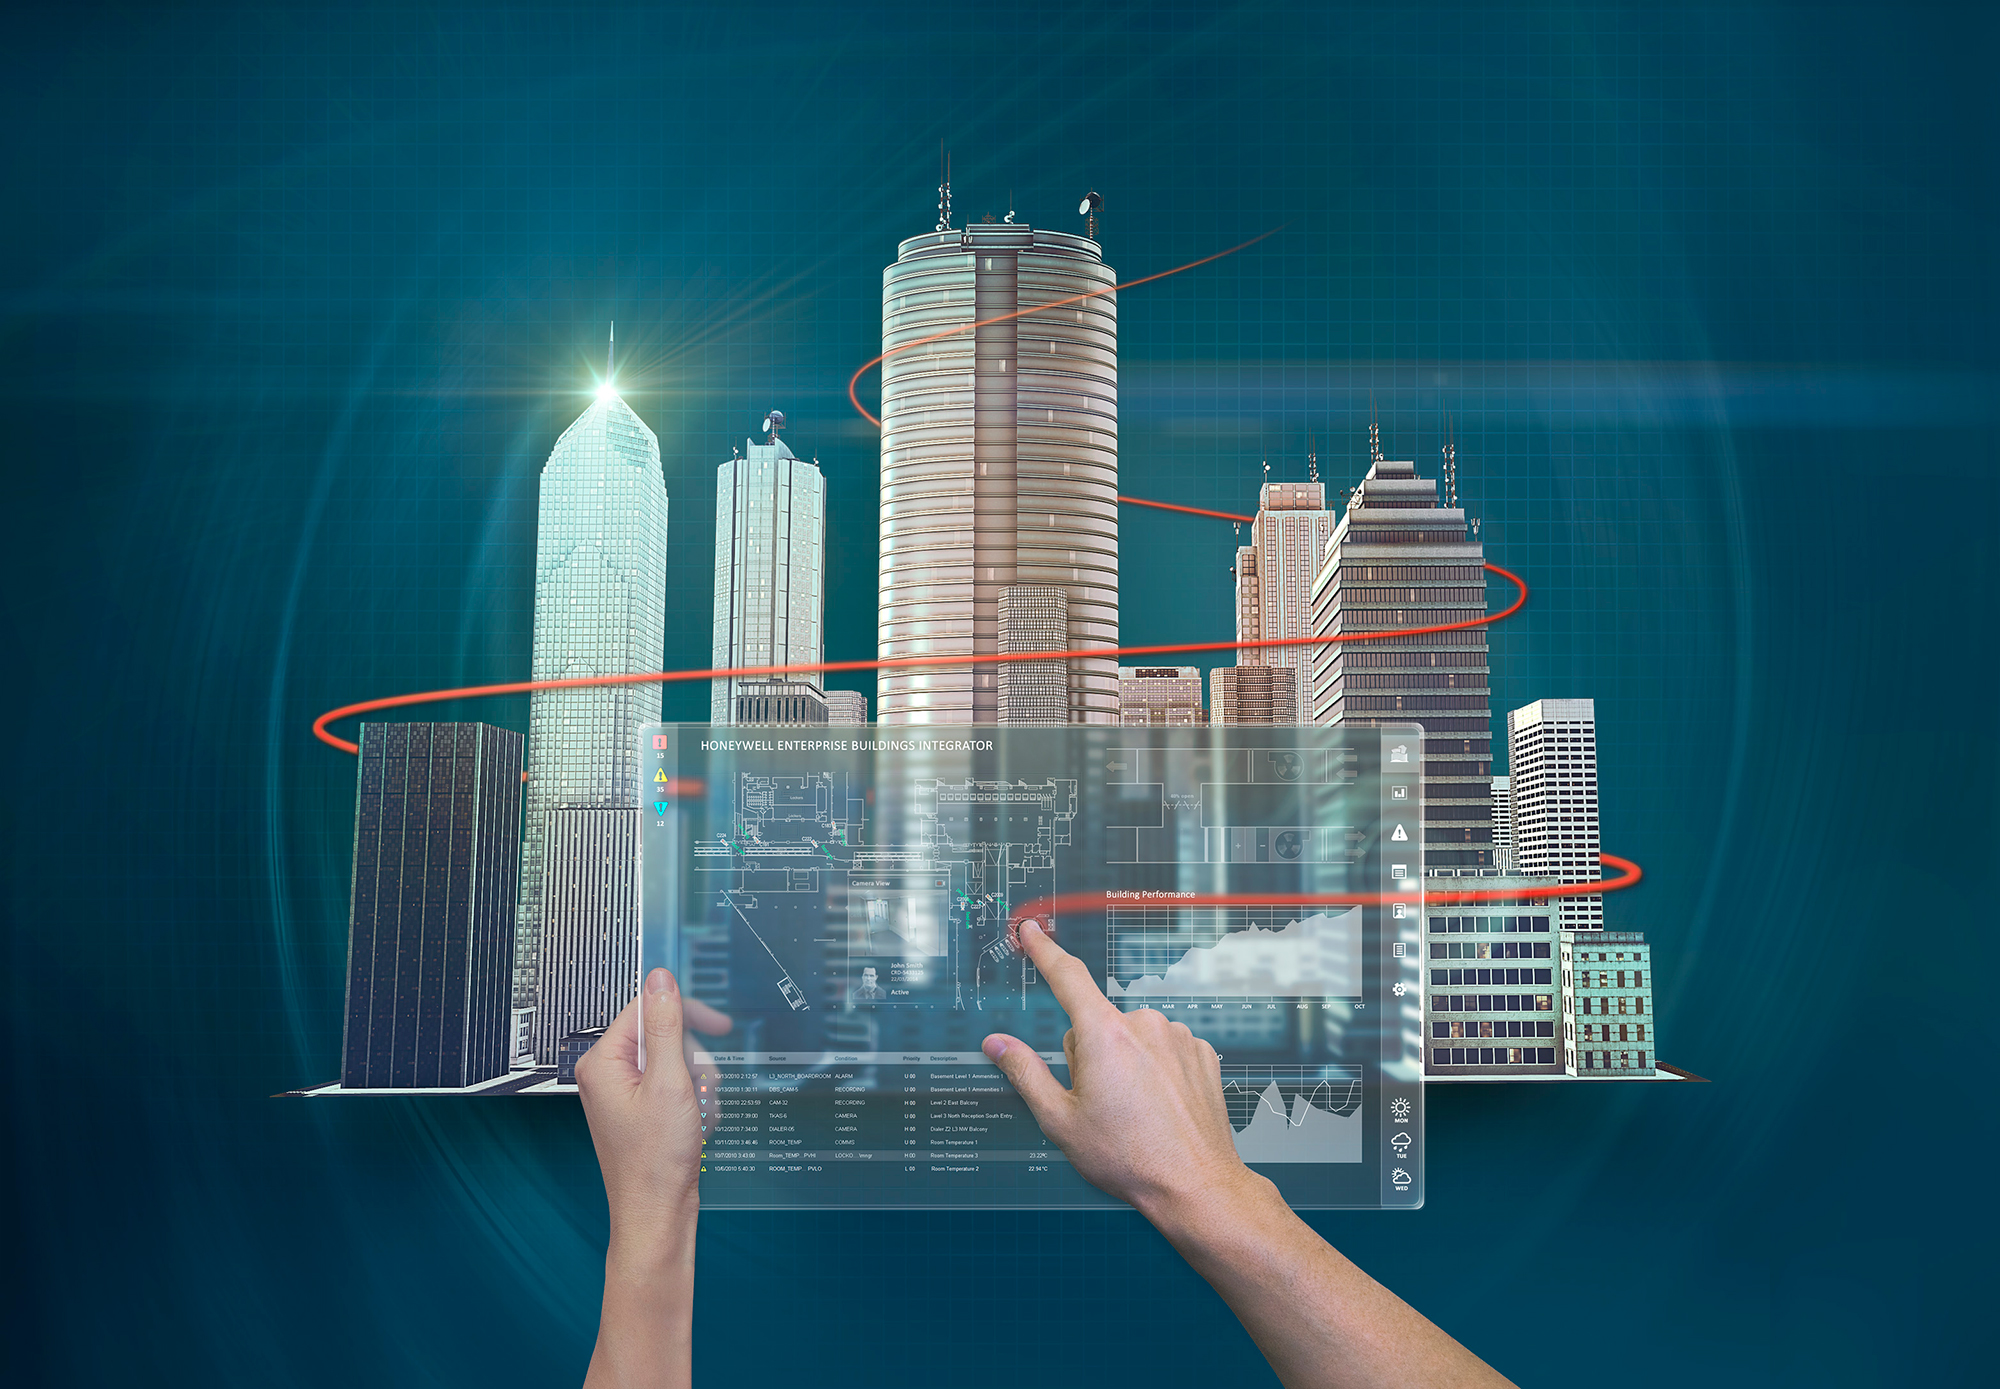
\includegraphics[width=45mm]{Figures/emmanuele_smartbuildings}
  \end{backgroundblock}
    \begin{backgroundblock}{10mm}{15mm}
    	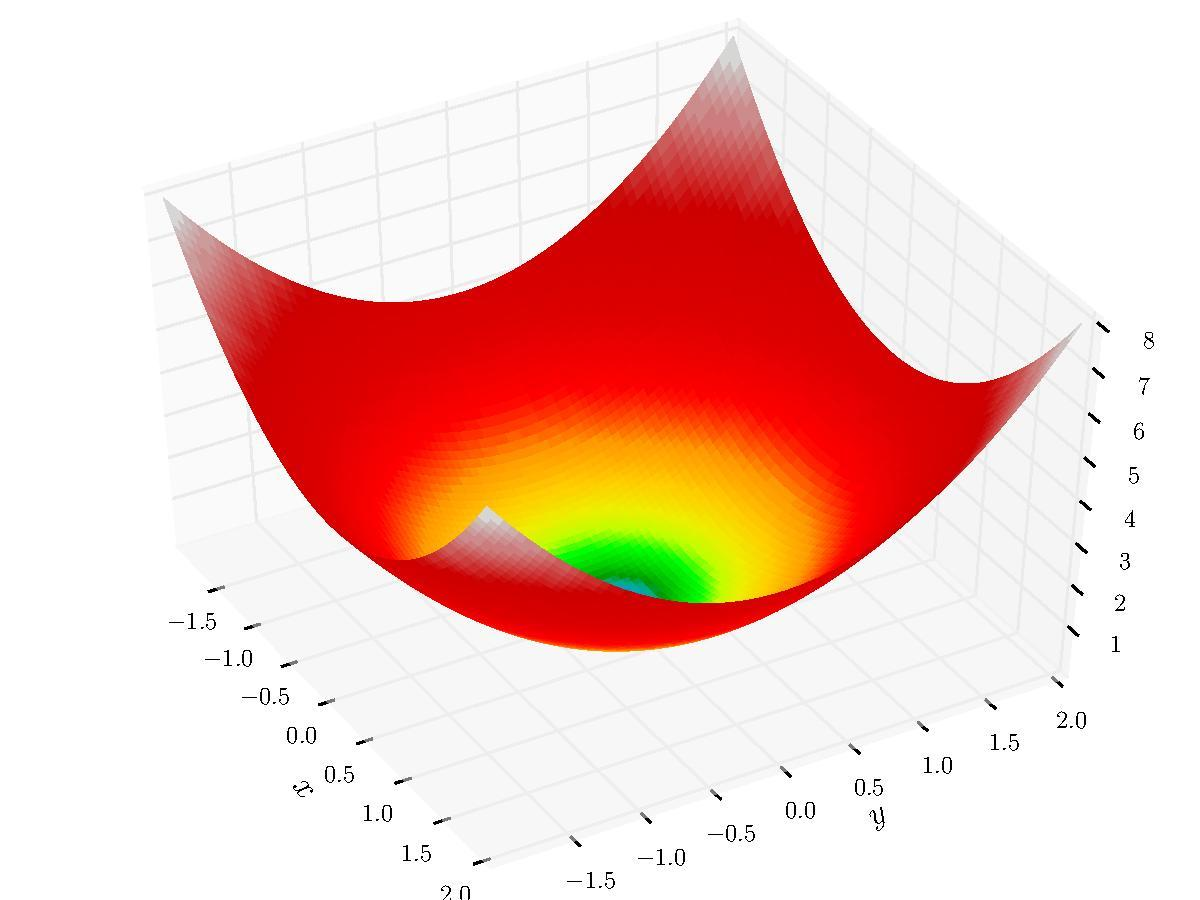
\includegraphics[width=45mm]{Figures/emanuele_convex}
    \end{backgroundblock}
    \begin{backgroundblock}{70mm}{15mm}
    	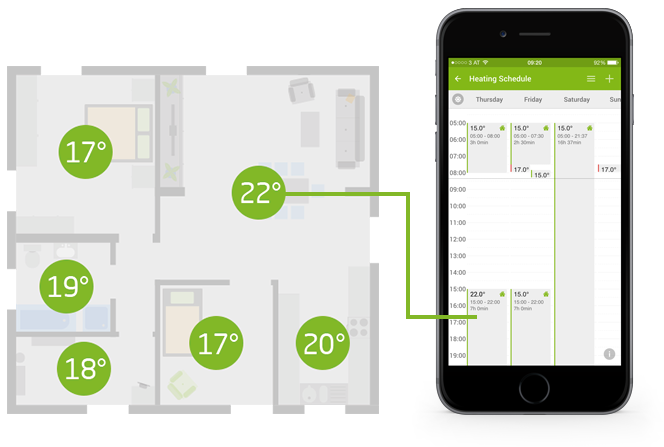
\includegraphics[width=45mm]{Figures/emanuele_others}
    \end{backgroundblock}
    \begin{backgroundblock}{10mm}{55mm}
    	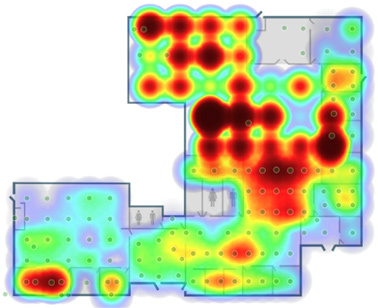
\includegraphics[width=45mm]{Figures/emanuele_idea}
    \end{backgroundblock}
\end{frame}
%%%%%%%%%%%%%%%%%%%%%%%%%%%%%%%%%%%%%%%%%%%%%%%%%%%%%%%%%%%%%%%%%%%%%%%%%%
\begin{frame}[t]{Objective}
	\begin{backgroundblock}{50mm}{30mm}
		
\includegraphics[width=30mm]{Figures/question}
	\end{backgroundblock}
\end{frame}

%%%%%%%%%%%%%%%%%%%%%%%%%%%%%%%%%%%%%%%%%%%%%%%%%%%%%%%%%%%%%%%%%%%%%%%%%%%%%
%\subsection{State of the art}
\begin{frame}[t]{Scope of the topic}
	\begin{itemize}
		\item Publications:
		\begin{itemize}
			\item Elsevier: Energy Conversion and Management
			\item Elsevier:Energy and Buildings
			\item Elsevier: Data Processing: Automated hotel systems
			\item IOS Press: Journal of Ambient Intelligence and Smart Environments
		\end{itemize}
		\item Books:
		\begin{itemize}
			\item Intelligent decisions
			\item Smart environments
		\end{itemize}
		\item Investment:
		\begin{itemize}
			\item EU (27\% - 2030)
			\item Smart environments: Tip of the iceberg
		\end{itemize}
		\item Robotics:
	\begin{itemize}
		\item Domotic effects
		\item Provider utility against local consumer management
	\end{itemize}
	\end{itemize}
\end{frame}
%%%%%%%%%%%%%%%%%%%%%%%%%%%%%%%%%%%%%%%%%%%%%%%%%%%%%%%%%%%%%%%%%%%%%%%%%%%%
\begin{frame}[t]{Real Questions}
	\begin{backgroundblock}{70mm}{20mm}
		
\includegraphics[width=45mm]{Figures/rocco_reality}
	\end{backgroundblock}
	\begin{itemize}
		\item
		Questions:
		\begin{itemize}
			\item Existing software?
			\item How does it work?
			\item Any rejections?
			\item Room assignment?
			\item Any optimisation used before?
			\item How to estimate your demand?
			\item Choice of prices?
			\item Maintenance costs?
		\end{itemize}
	\end{itemize}
\begin{backgroundblock}{25mm}{53mm}
	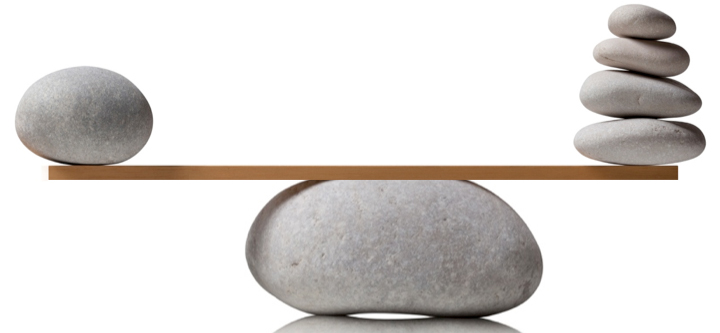
\includegraphics[width=75mm]{Figures/rocco_quality}
\end{backgroundblock}
\end{frame}

%\begin{frame}{Pumping cycle: Detail}
%	\begin{backgroundblock}{10mm}{20mm}
%		\includegraphics[width=110mm]{Figures/pumping_cycle.png}
%	\end{backgroundblock}
%	\begin{backgroundblock}{10mm}{83mm}
%		\scriptsize Fig. 3 Pumping cycle simulation (Greg Horn)
%	\end{backgroundblock}
%\end{frame}
%%%%%%%%%%%%%%%%%%%%%%%%%%%%%%%%%%%%%%%%%%%%%%%%%%%%%%%%%%%%%%%%%%%%%%%%%%%%%%%%%

\begin{frame}[t]{Real Answers: Genova}
	
	\begin{columns}
		\begin{column}{0.5\textwidth}
				\begin{itemize}
					\item
					Estimation of demand?
					\begin{itemize}
						\item Not generally
						\item Prefer external analysis
					\end{itemize}
				\end{itemize}
				\begin{itemize}
					\item Room assignment?
						\begin{itemize}
							\item Random
							\item Based on client assignment
						\end{itemize}
				\end{itemize}
				\begin{backgroundblock}{15mm}{60mm}
					
\includegraphics[width=45mm]{Figures/rocco_istat}
				\end{backgroundblock}
		\end{column}
		\begin{column}{0.5\textwidth}  %%<--- here
				\begin{itemize}
					\item
					Optimisation ever used?
					\begin{itemize}
						\item A few aware of profit optimisation
						\item Absolutly no energy involvement
					\end{itemize}
				\end{itemize}
				\begin{backgroundblock}{70mm}{50mm}
					
\includegraphics[width=45mm]{Figures/rocco_software}
				\end{backgroundblock}
		\end{column}
	\end{columns}

\end{frame}
%%%%%%%%%%%%%%%%%%%%%%%%%%%%%%%%%%%%%%%%%%%%%%%%%%%%%%%%%%%%%%%%%%%%%%%%%%%%%%
\section{Modelling}
\begin{frame}{Basic principle up to the first order}
	\begin{backgroundblock}{70mm}{50mm}
		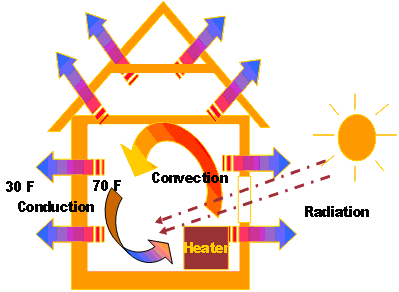
\includegraphics[width=55mm]{Figures/emanueleHeatTransfer}
	\end{backgroundblock}
	\begin{align*}
	& q_{tot_{t}} = \Sigma q_{k_{t}} + \Sigma q_{h_{t}} + \Sigma q_{vent_{t}} + \Sigma q_{sun_{t}} + q_{pump_{t}} \\
	& q_{tot_{t}} = \rho V c_{p} \frac{d T}{d t} \numberthis
	\label{eq:model}
	\end{align*}
	\begin{enumerate}
		\item Blueprint approach
		\item Parameter identification \\
		(reality or simulation)
	\end{enumerate}
	\begin{itemize}
		\item Norm: UNI/TS 11300 (20$\pm$2 $^{\circ}$C)
	\end{itemize}
\end{frame}
%%%%%%%%%%%%%%%%%%%%%%%%%%%%%%%%%%%%%%%%%%%%%%%%%%%%%%%%%%%%%%%%%%%%%%%%%%%%%%
%\subsection{Previous analysis}
\begin{frame}{Blueprint: Generality}
	\begin{columns}
		\begin{column}{0.5\textwidth}
			\begin{itemize}
				\item Parameters: Dimensional characteristics\\
				and thermal characteristics
			\end{itemize}
		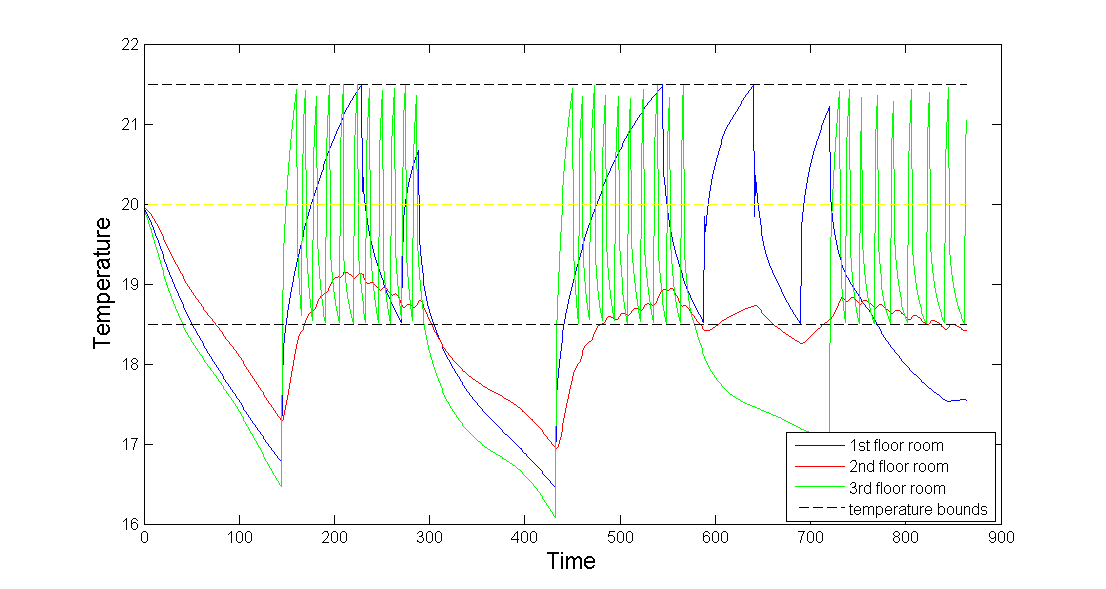
\includegraphics[width=65mm]{Figures/temperature_anal}
		\end{column}
		\begin{column}{0.5\textwidth}
			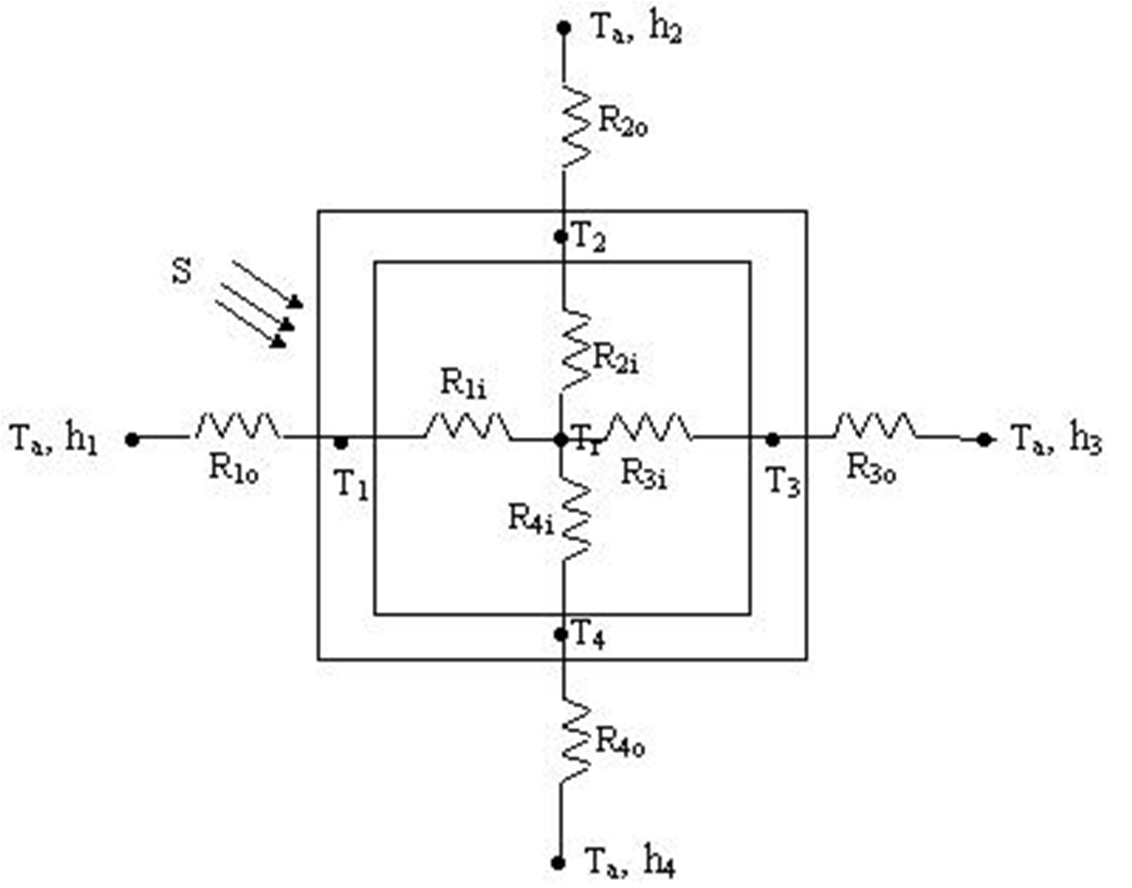
\includegraphics[width=60mm]{Figures/emanuelelumped_parameter}
			\begin{itemize}
			\item Control proposal: ON-OFF Controller
			\item Adjacency proposal: Lumped parameter
			\end{itemize}
		\end{column}
	\end{columns}
\end{frame}

%%%%%%%%%%%%%%%%%%%%%%%%%%%%%%%%%%%%%%%%%%%%%%%%%%%%%%%%%%%%%%%%%%%%%%%%%%%%%%%%
\begin{frame}{Blueprints proposed}
	\begin{columns}
		\begin{column}{0.25\textwidth}
			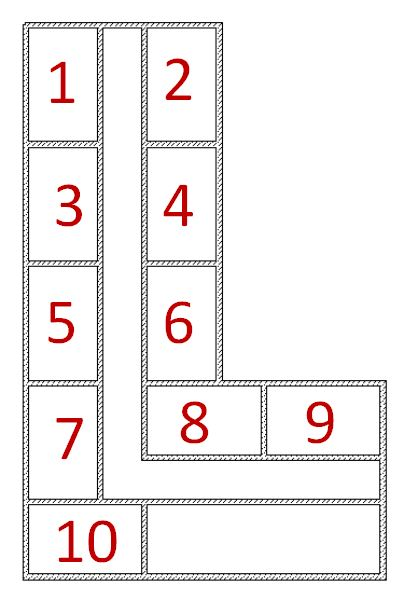
\includegraphics[width=35mm]{Figures/emanuele1_f_hotel}\\
			\centering Hotel 1
		\end{column}
		\begin{column}{0.75\textwidth}
			\centering
			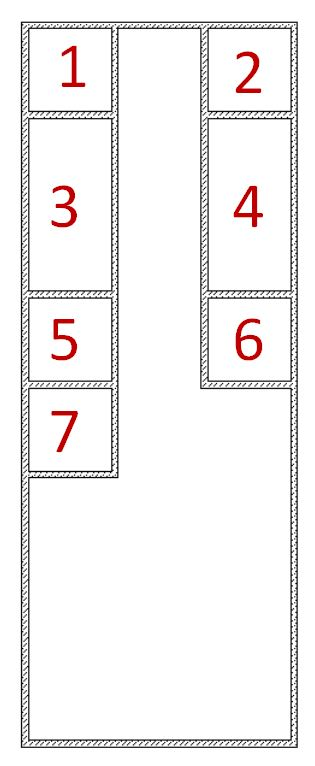
\includegraphics[width=21mm]{Figures/emanuele3_f_hotel_1}
			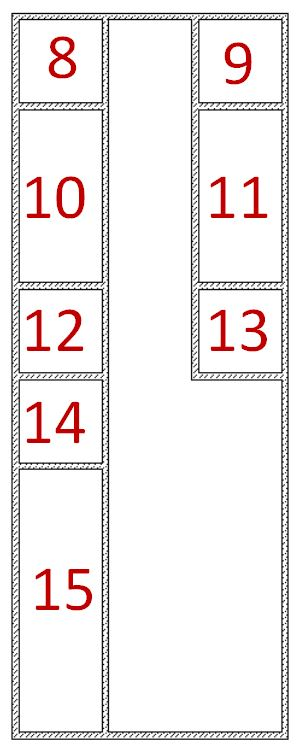
\includegraphics[width=20mm]{Figures/emanuele3_f_hotel_2}
			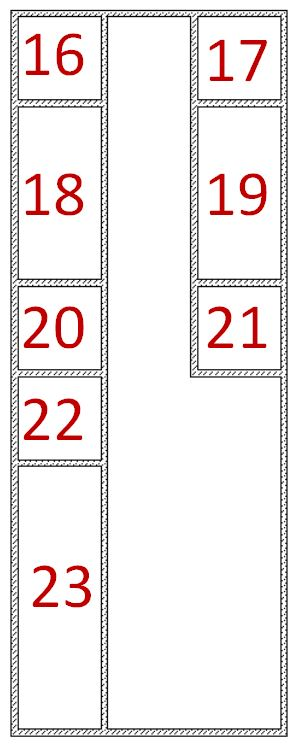
\includegraphics[width=20mm]{Figures/emanuele3_f_hotel_3}\\
			\centering Hotel 2	
		\end{column}
	\end{columns}
\end{frame}
%%%%%%%%%%%%%%%%%%%%%%%%%%%%%%%%%%%%%%%%%%%%%%%%%%%%%%%%%%%%%%%%%%%%%%%%%%%%%%%%
%\subsection{Parameter identification}
\begin{frame}{Parameter Identification}	
	\begin{backgroundblock}{10mm}{75mm}
		
\includegraphics[width=15mm]{Figures/matlab_logo}
	\end{backgroundblock}
	\begin{columns}
			\begin{column}{0.5\textwidth}
			\tiny	\begin{align*}
					& \hat{T}_{i,t+1}=\frac{1}{c_i}\left[\sum_{i\sim j\bigcup e}(\hat{T}_{i,t}-\hat{T}_{j,t})+K_{u}u_{i,t}+q^S_{i,t}+\hat{T}_{i,t}\right]+S_p\\
					& u_{i,t}=u_{i,t-1}+K_{u,i}(e_{i,t}-e_{i,t-1})\\
					& e_{i,t} = T_{sp,t}-T_{i,t}\\
					& \forall i \mid 0=1...n_r\\
					& \forall t \mid t=1...P \numberthis
				\end{align*}
				\begin{equation}
					\begin{array}{rlclcl}
					\displaystyle \theta^*=\arg \min_{\theta\in\mathbb{R}} & \multicolumn{3}{l}{(T_{i,t}-\hat{T}_{i,t})^2} \\
					\textrm{s.t.} & \theta \geq 0 \\
					& S_p = 0\\
					\end{array}
					\label{eq:opt_k_cluster}
				\end{equation}	\normalsize	
			\end{column}
		\begin{column}{0.5\textwidth}  %%<--- here
			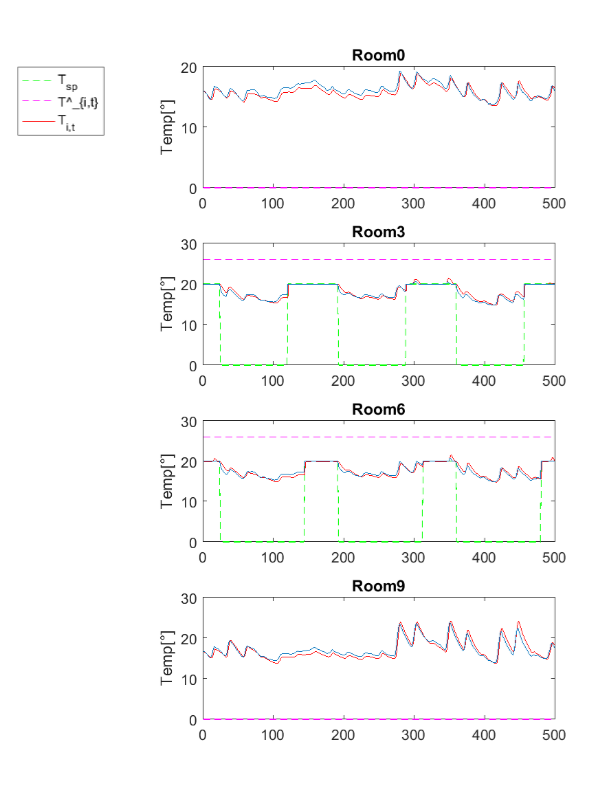
\includegraphics[width=55mm]{Figures/Sys_ID}
		\end{column}
	\end{columns}
\end{frame}
%%%%%%%%%%%%%%%%%%%%%%%%%%%%%%%%%%%%%%%%%%%%%%%%%%%%%%%%%%%%%%%%%%%%%%%%%%%%%%%%
\section{Optimisation}
\begin{frame}[t]{Rooms Assignment Problem}
		\begin{backgroundblock}{10mm}{40mm}
			
\includegraphics[width=25mm]{Figures/ernesto_gurobi}
		\end{backgroundblock}
		\begin{columns}
			\begin{column}{0.4\textwidth}
				\centering
				\scriptsize	
				\begin{flalign*}
				&\begin{array}{rlclcl}
				\displaystyle Y^*=\max_{x_{d,r}} & \multicolumn{3}{l}{\sum_{d\in D}\sum_{r\in R_d}Y_{d,r}x_{d,r}} \\
				\textrm{s.t.} & \sum_{r\in R_{dn}}x_{d,r}=1 \text{ }\forall d\in D \\
				& x_{d,r}+x_{k,r}\leq 1 \text{ } \forall d\in D\text{, }\forall k\in D_d\\
				& \text{ and } \forall r\in R_d\cap R_k
				\end{array}\\
				\end{flalign*}
					
				\begin{table}[htbp]
					\centering
					\caption{Levels of daily profits used as a marketing strategy $Y_{d,r}$}
					\begin{tabular}{cr|ccc}
						\toprule
						\multicolumn{2}{c|}{\multirow{2}[0]{*}{Request}} & \multicolumn{3}{c}{Room type} \\
						\multicolumn{2}{c|}{} & Low  & Medium & High \\ 
						\midrule
						\multirow{2}[0]{*}{} & Low &   9   &   7    & 2 \\
						& Medium &   0    &   22    &  17\\
						& High &0 & 0& 72\\
						\bottomrule
					\end{tabular}%
					\label{tab:profits}%
				\end{table}\normalsize	%
			\end{column}

			\begin{column}{0,4\textwidth}
				\centering
				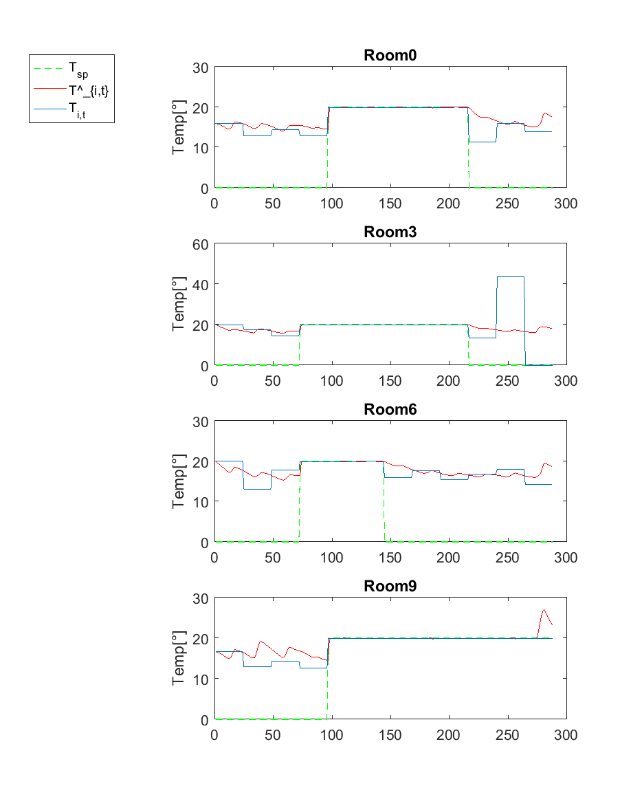
\includegraphics[width=55mm]{Figures/ernesto_Validation}
			\end{column}
		\end{columns}
\end{frame}
%%%%%%%%%%%%%%%%%%%%%%%%%%%%%%%%%%%%%%%%%%%%%%%%%%%%%%%%%%%%%%%%%%%%%%%%%%%%%%%
\begin{frame}[t]{Energy optimisation problem}
	
	\begin{columns}
		\begin{column}{0.3\textwidth}
			\scriptsize	
			\begin{flalign*}
			&\begin{array}{rlclcl}
			\displaystyle E^*=\min_{x_{d,r}} & \multicolumn{3}{l}{\sum_{t\in T}\sum_{i\in R}u_{i,t}} \\
			\textrm{s.t.} & \sum_{r\in R_{dn}}x_{d,r}=1 \text{ }\forall d\in D \\
			& x_{d,r}+x_{k,r}\leq 1 \text{ } \forall d\in D\text{, }\forall k\in D_d\\
			& \text{ and } \forall r\in R_d\cap R_k\\
			& z_{i,t} = \sum_{\substack{d\in D\\t_d^{in}\leq t \leq t_d^{out}}} x_{d,r} \text{ } \forall r\in R \text{, }\\
			&\forall t\in{T_1}\\ 
			& \hat{T}_{i,t+1}=\frac{1}{c_i}(\sum_{i\sim j\bigcup e}(\hat{T}_{i,t}-\hat{T}_{j,t})\\
			& \qquad \qquad +K_{u}u_{i,t}+q^S_{i,t}+\hat{T}_{i,t})\\
			& T_{i,1} = \hat{T}_{i,1}\\
			& u_{i,t}\geq 0\\
			& u_{i,t}\geq (T_{sp}-T_{i,t})-M(1-z_{i,t})\\
			& z_{j,t} \geq z_{j,t}\geq 1-M(1-z_{k,t}) \text{ }\forall j\in{R_{s}} \text{ and }k\sim j\\
			& Y_{t}\geq Y^*
			\end{array}\\
			& \numberthis
			\label{eq:opt_multi}
			\end{flalign*}
		\end{column}
		\begin{column}{0.1\textwidth}  %%<--- here
			
		\end{column}
		\begin{column}{0,5\textwidth}
			\centering
			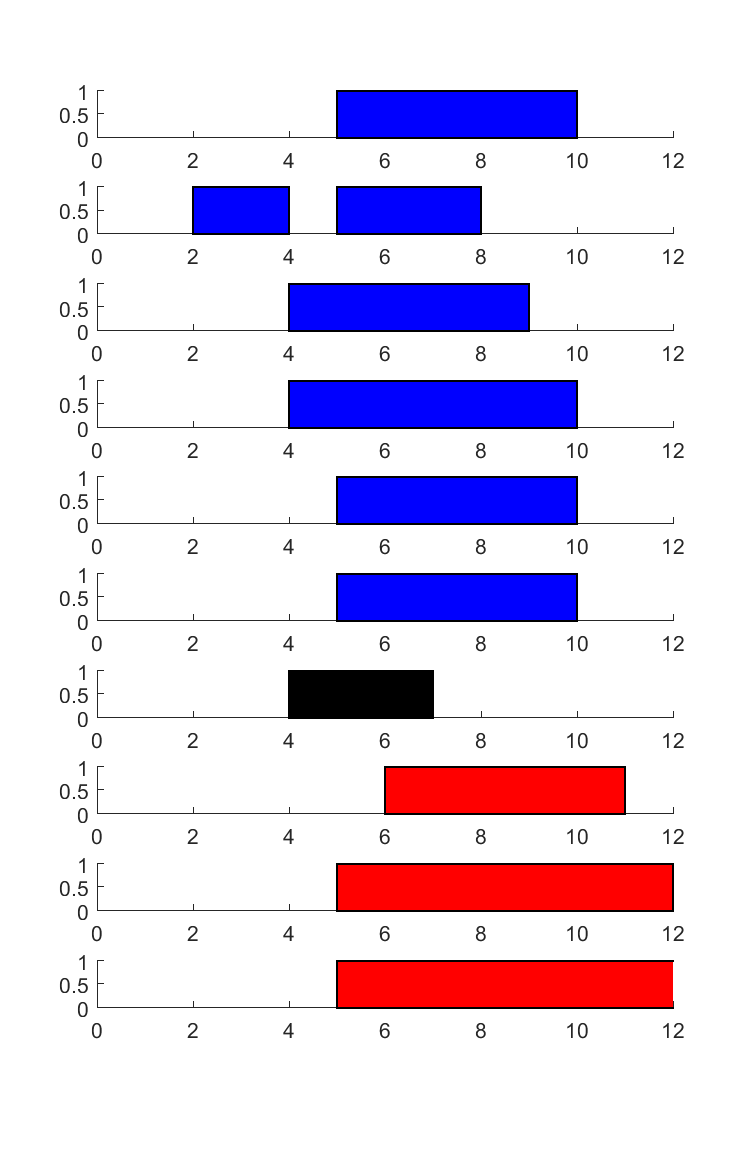
\includegraphics[width=50mm]{Figures/ernesto_rooms}
		\end{column}
	\end{columns}
\end{frame}
%%%%%%%%%%%%%%%%%%%%%%%%%%%%%%%%%%%%%%%%%%%%%%%%%%%%%%%%%%%%%%%%%%%%%%%%%%%%%%%%
\section{Experiments, results and discussion}
%\subsection{Experimental campaign}
\begin{frame}{Instances generation}
	\begin{columns}
		\begin{column}{0.45\textwidth}
			\begin{itemize}
				\item Demand:
				\begin{itemize}
					\item 30\%
					\item 50\%
					\item 65\%
				\end{itemize}
				\item Types of rooms:
				\begin{itemize}
					\item High:10\%
					\item Medium:30\%
					\item Basic:60\%
				\end{itemize}
				\item 10 instances used:
				\begin{itemize}
					\item Revenue optimisation
					\item 5: Equivalent revenue solutions
					\item 1: Energy consumption minimisation
				\end{itemize}
				\item Time horizon: 14 days
				\item Figure of merit: RPD
			\end{itemize}			
		\end{column}
		\begin{column}{0.55\textwidth}
			\centering
			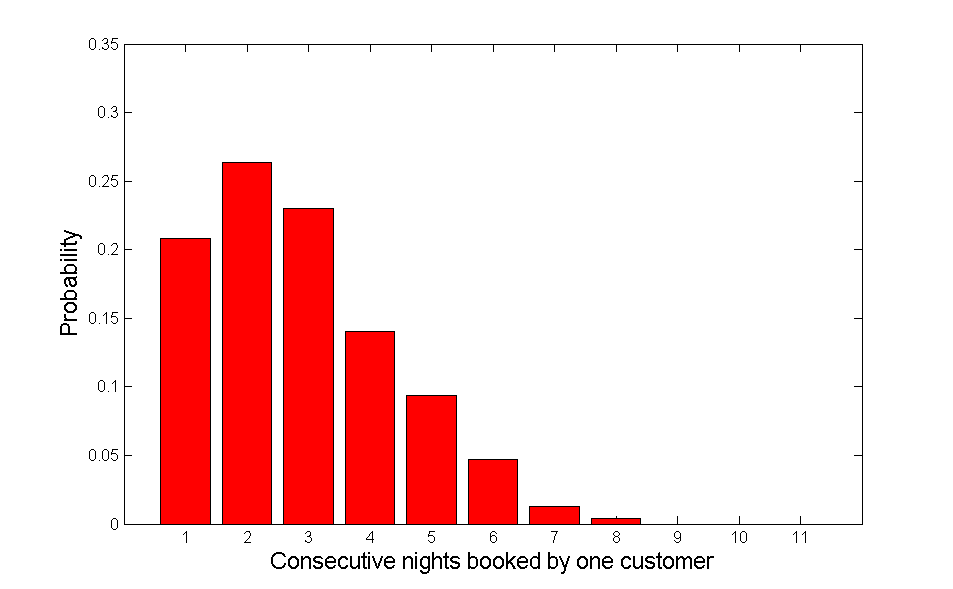
\includegraphics[width=70mm]{Figures/Booking_probability1}			
		\end{column}
	\end{columns}		
\end{frame}
%%%%%%%%%%%%%%%%%%%%%%%%%%%%%%%%%%%%%%%%%%%%%%%%%%%%%%%%%%%%%%%%%%%%%%%%%%%%%%%
%\subsection{Results and Conclusion}
\begin{frame}{Hotel 1: Final occupancy}
	\begin{columns}
		\begin{column}{0.33\textwidth}		
			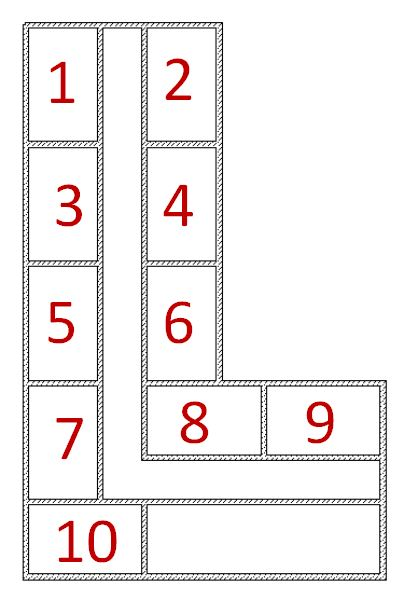
\includegraphics[width=35mm]{Figures/emanuele1_f_hotel}
		\end{column}
		\begin{column}{0.33\textwidth}  %%<--- here
			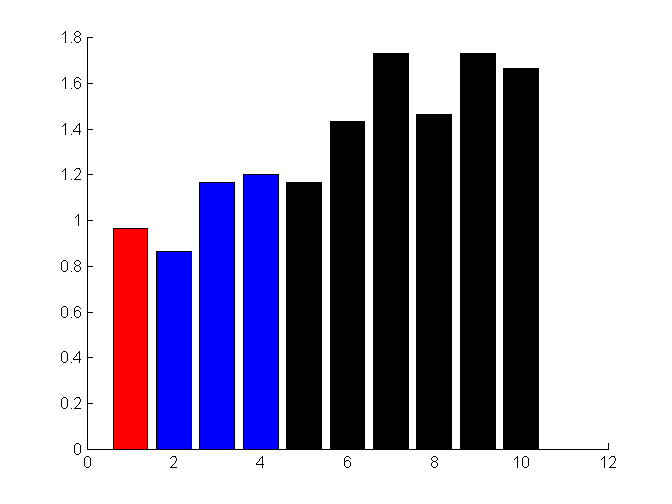
\includegraphics[width=35mm]{Figures/emanuele10_opt}\\
			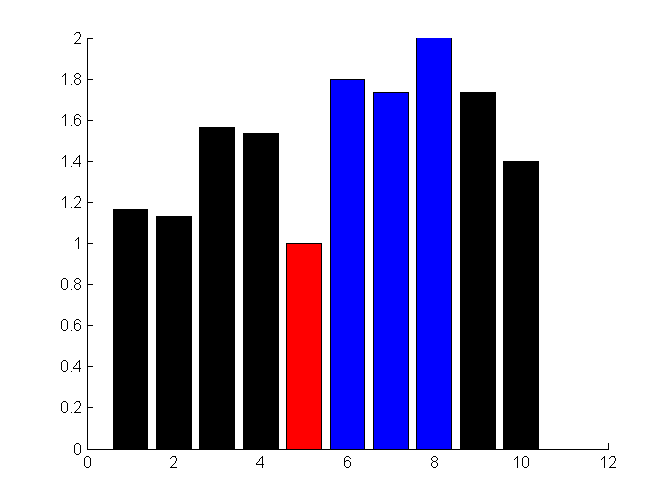
\includegraphics[width=35mm]{Figures/emanuele10_opt_half}
		\end{column}
		\begin{column}{0.33\textwidth}  %%<--- here
			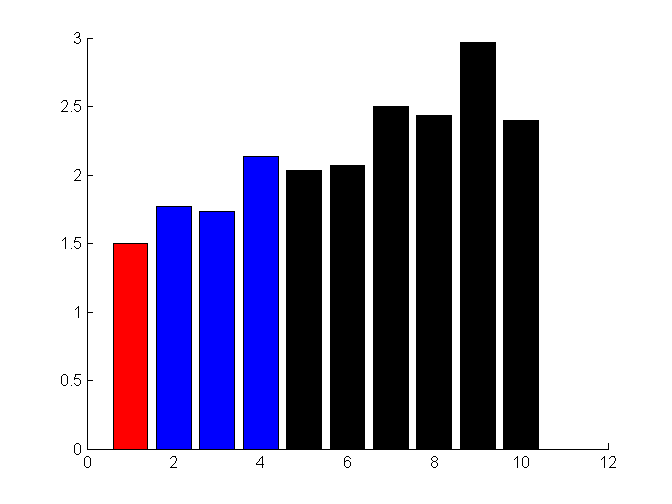
\includegraphics[width=35mm]{Figures/emanuele10_not_opt}\\
			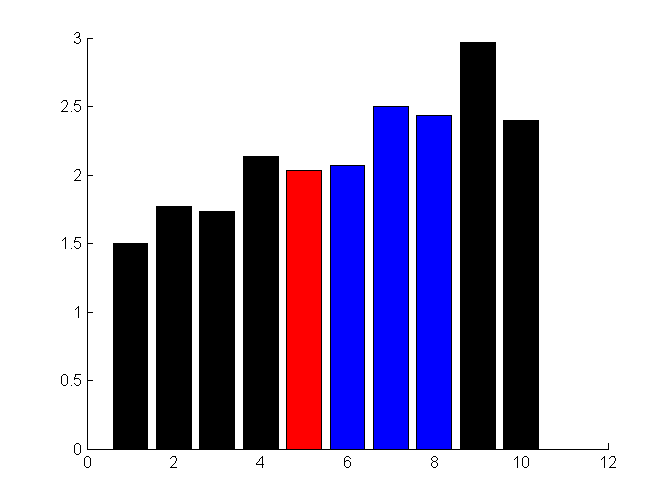
\includegraphics[width=35mm]{Figures/emanuele10_not_opt_half}
		\end{column}
	\end{columns}
		\begin{backgroundblock}{30mm}{80mm}
			\centering
			
\includegraphics[width=100mm]{Figures/classes}
		\end{backgroundblock}		
\end{frame}
%%%%%%%%%%%%%%%%%%%%%%%%%%%%%%%%%%%%%%%%%%%%%%%%%%%%%%%%%%%%%%%%%%%%%%%%%%%%%%
\begin{frame}{Hotel 2: Final occupancy}
	\begin{backgroundblock}{20mm}{20mm}
		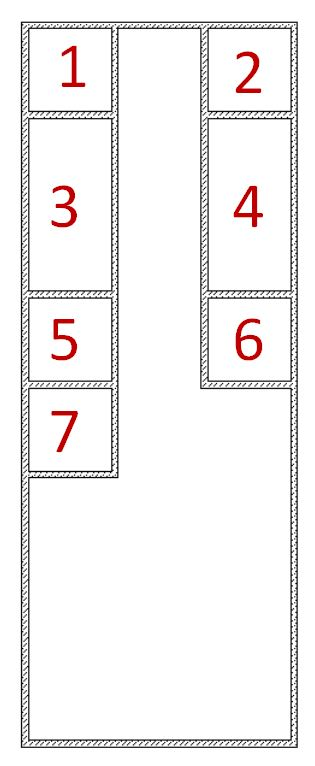
\includegraphics[width=16mm]{Figures/emanuele3_f_hotel_1}
	\end{backgroundblock}
	\begin{backgroundblock}{55mm}{20mm}
		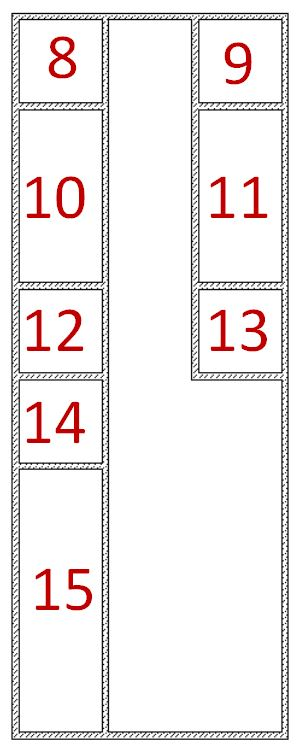
\includegraphics[width=15mm]{Figures/emanuele3_f_hotel_2}
	\end{backgroundblock}
	\begin{backgroundblock}{90mm}{20mm}
		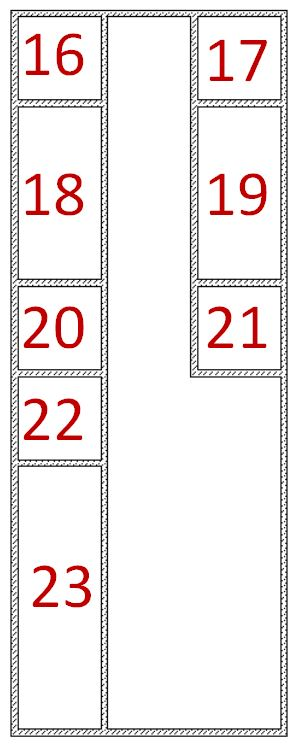
\includegraphics[width=15mm]{Figures/emanuele3_f_hotel_3}
	\end{backgroundblock}
	\begin{backgroundblock}{15mm}{60mm}
		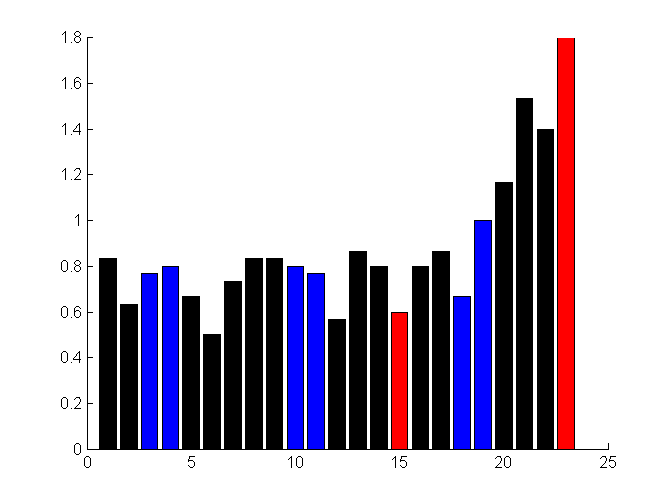
\includegraphics[width=45mm]{Figures/emanuele23_opt}
	\end{backgroundblock}
	\begin{backgroundblock}{70mm}{60mm}
		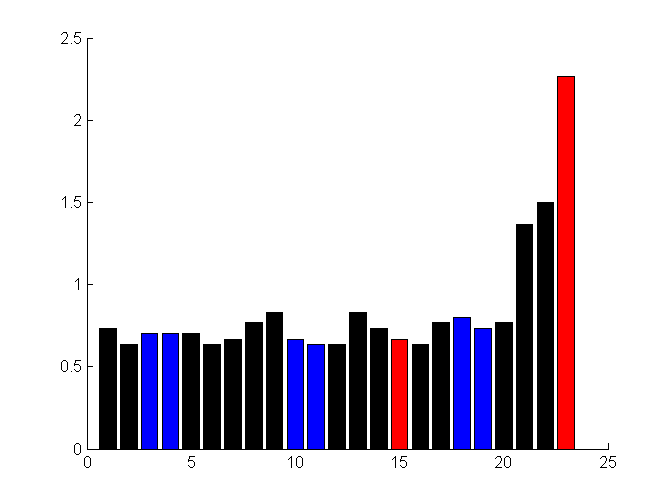
\includegraphics[width=45mm]{Figures/emanuele23_not_opt}
	\end{backgroundblock}
\end{frame}
%%%%%%%%%%%%%%%%%%%%%%%%%%%%%%%%%%%%%%%%%%%%%%%%%%%%%%%%%%%%%%%%%%%%%%%%%%%%%%%
\begin{frame}{RPD and Conclusions}	
	\begin{columns}
		\begin{column}{0.5\textwidth}		
			\begin{table}[htbp]
				\caption{Relative percentage difference (RPD)}
				\label{Table_RPD}
				\begin{tabular}{lllll}
					& 30\% & 50\% & 65\% &  \\
					Hotel 1.1 & 5.2  & 6.7  & 5.6  &  \\
					Hotel 1.2  & 2.9  & 9.5  & 5.2  &  \\
					Hotel 2.1    & 2.7  & 1.5  & 1.7  & 
				\end{tabular}
			\end{table}
		\end{column}
		\begin{column}{0.5\textwidth}  %%<--- here
			\begin{itemize}
				\item Energy optimisation:
				\begin{itemize}
					\item Biased to maximal revenue
					\item Clustering growing solutions in time prefered
				\end{itemize}
				\item Savings:
				\begin{itemize}
					\item Structural dependence
					\item Orientation to the sun
				\end{itemize}
				\item Proposal:
				\begin{itemize}
					\item High level rooms in warmest locations
				\end{itemize}
			\end{itemize}
		\end{column}
	\end{columns}
\end{frame}
%%%%%%%%%%%%%%%%%%%%%%%%%%%%%%%%%%%%%%%%%%%%%%%%%%%%%%%%%%%%%%%%%%%%%%%%%%%%%
\begin{frame}{}
		\centering \Large
		\emph{THANK YOU FOR YOUR ATTENTION}\\
		
\includegraphics[width=45mm]{Figures/ernesto_gurobi}
\end{frame}
\end{document}
%%%%%%%%%%%%%%%%%%%%%%%%%%%%%%%%%%%%%%%%%%%%%%%%%%%%%%%%%%%%%%%%%%%%%%%%%%%%%%

